On considère la fonction $f$ définie sur $]0\ ;\ +\infty[$ et sa courbe représentative $C_f$.
La droite $T_A$ est tangente à $C_f$ au point $A(1\ ;\ 20)$ et passe par le point $B(3\ ;\ 10)$.

\begin{enumerate}
\item \begin{enumerate}
\item Le point $A(1\ ;\ 20)$ appartient à la courbe $C_f$.

Donc l'image de $1$ par $f$ est l'ordonnée du point $A$ :
\[
f(1)=20.
\]
\item La droite $T_A$ est tangente à la courbe $C_f$ au point d'abscisse $1$.

Le nombre dérivé $f'(1)$ est donc le coefficient directeur de cette tangente.
Comme $T_A$ passe par les points $A(1\ ;\ 20)$ et $B(3\ ;\ 10)$, on a :
\begin{align*}
	f'(1)&=\frac{y_B-y_A}{x_B-x_A}\\
	&=\frac{10-20}{3-1}\\
	&=\frac{-10}{2}\\
	&=-5.
\end{align*}

Ainsi,
\[
f'(1)=-5.
\]
\item La droite $T_A$ est tangente à la courbe $C_f$ au point d'abscisse $1$.

Son équation est :
\begin{align*}
y&=f'(1)(x-1)+f(1)\\
y&=-5(x-1)+20\\
y&=-5x+15
\end{align*}

L'équation réduite de la tangente $T_A$ à $C_f$ au point $A$ est donc bien :
\[
y=-5x+25.
\]
\end{enumerate}

\item Pour la suite, on a, pour tout $x\in]0\ ;\ +\infty[$,
\[
f(x)=\frac{4x^2+7x+9}{x}.
\]

\begin{enumerate}
\item Pour tout $x\in]0\ ;\ +\infty[$, on a :
$$
f(x)=\frac{4x^2+7x+9}{x}.
$$

On pose, pour tout $x\in]0\ ;\ +\infty[$ :
$$
u(x)=4x^2+7x+9
\qquad \text{et} \qquad
v(x)=x.
$$

Ainsi :
$$
f=\frac{u}{v}.
$$

Les fonctions $u$ et $v$ sont dérivables sur $]0\ ;\ +\infty[$, et, pour tout $x\in]0\ ;\ +\infty[$ :
$$
u'(x)=8x+7
\qquad \text{et} \qquad
v'(x)=1.
$$

De plus, pour tout $x\in]0\ ;\ +\infty[$, on a $v(x)=x\neq 0$.

On peut donc appliquer la formule de dérivation d’un quotient :
$$
\left(\frac{u}{v}\right)'=\frac{u'v-uv'}{v^2}.
$$

Ainsi, pour tout $x\in]0\ ;\ +\infty[$ :
\begin{align*}
	f'(x)
	&=\frac{u'(x)v(x)-u(x)v'(x)}{\left(v(x)\right)^2}\\
	&=\frac{(8x+7)\times x-(4x^2+7x+9)\times 1}{x^2}\\
	&=\frac{8x^2+7x-4x^2-7x-9}{x^2}\\
	&=\frac{4x^2-9}{x^2}\\
	&=\frac{(2x-3)(2x+3)}{x^2}.
\end{align*}

Donc, pour tout $x\in]0\ ;\ +\infty[$,
$$
f'(x)=\frac{(2x-3)(2x+3)}{x^2}.
$$


\item On étudie le signe de
$$
f'(x)=\frac{(2x-3)(2x+3)}{x^2}
$$
sur $]0\ ;\ +\infty[$.

Pour tout $x\in]0\ ;\ +\infty[$, on a :
\[
x^2>0.
\]

De plus, comme $x>0$, alors :
\[
2x+3>0.
\]

Le signe de $f'(x)$ est donc le signe de $2x-3$.\\
Or :
$
2x-3<0 \iff x<\frac{3}{2}$



Ainsi :
\begin{itemize}[left=5mm,label={\textbullet~~}]
\item $f'(x)<0$ sur $\left]0\ ;\ \dfrac{3}{2}\right[$ ;
\item $f'\left(\dfrac{3}{2}\right)=0$ ;
\item $f'(x)>0$ sur $\left]\dfrac{3}{2}\ ;\ +\infty\right[$.
\end{itemize}

\item On en déduit les variations de $f$ sur $]0\ ;\ +\infty[$.

Comme $f'(x)<0$ sur $\left]0\ ;\ \dfrac{3}{2}\right[$, la fonction $f$ est décroissante sur cet intervalle.

Comme $f'(x)>0$ sur $\left]\dfrac{3}{2}\ ;\ +\infty\right[$, la fonction $f$ est croissante sur cet intervalle.

De plus :
\begin{align*}
	f\left(\frac{3}{2}\right)
	&=\frac{4\left(\frac{3}{2}\right)^2+7\left(\frac{3}{2}\right)+9}{\frac{3}{2}}\\
	&=\frac{9+\frac{21}{2}+9}{\frac{3}{2}}\\
	&=\frac{\frac{57}{2}}{\frac{3}{2}}\\
	&=19.
\end{align*}

On peut résumer ces résultats dans le tableau de variations suivant :

\begin{center}
	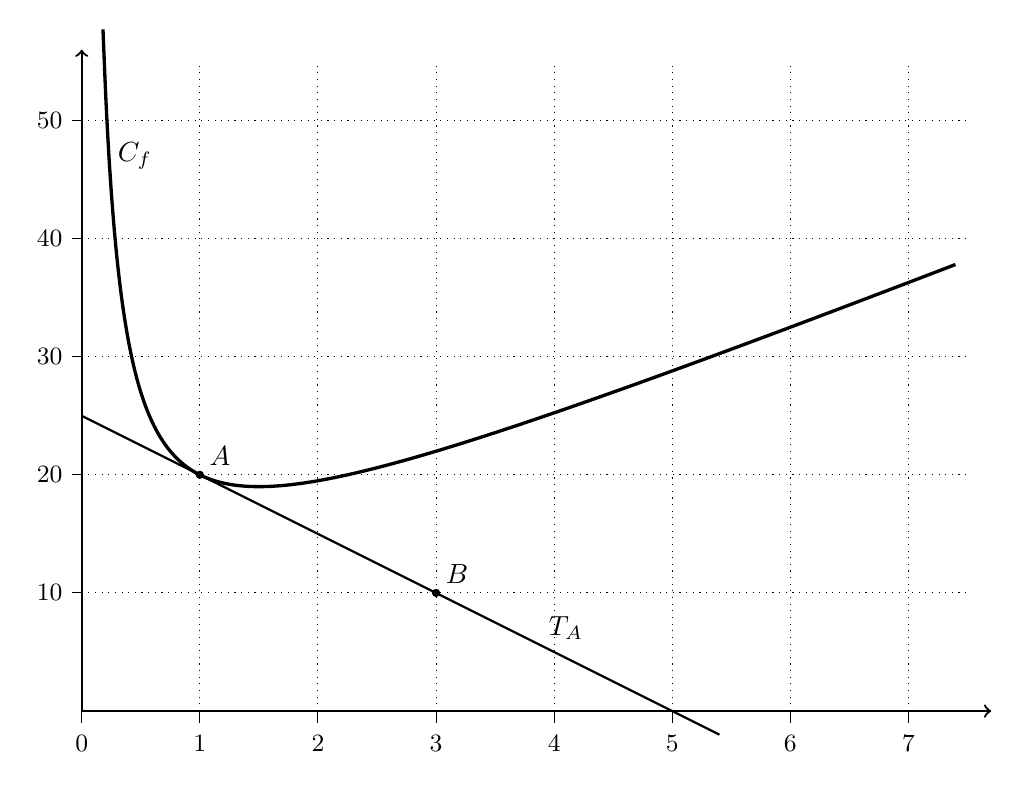
\begin{tikzpicture}[x=1.5cm,y=0.15cm]
		
		
		
		
		
		\foreach \x in {0,1,2,3,4,5,6,7}
		{
			\draw[dotted] (\x,0) -- (\x,55);
		}
		
		
		\foreach \y in {0,10,20,30,40,50}
		{
			\draw[dotted] (0,\y) -- (7.5,\y);
		}
		
		
		\draw[->,thick] (0,0) -- (7.7,0);
		\draw[->,thick] (0,0) -- (0,56);
		
		
		\foreach \x in {0,1,2,3,4,5,6,7}
		{
			\draw (\x,0) -- (\x,-1);
			\node[below] at (\x,-1.2) {\small $\x$};
		}
		
		
		\foreach \y in {10,20,30,40,50}
		{
			\draw (0,\y) -- (-0.08,\y);
			\node[left] at (-0.08,\y) {\small $\y$};
		}
		
		
		\draw[very thick, domain=0.18:7.4, samples=300, smooth, variable=\x]
		plot ({\x},{(4*\x*\x+7*\x+9)/\x});
		
		
		\draw[thick, domain=0:5.4, samples=2, variable=\x]
		plot ({\x},{-5*\x+25});
		
		
		\fill (1,20) circle (1.5pt);
		\fill (3,10) circle (1.5pt);
		
		
		\node[above right] at (1,20) {$A$};
		\node[above right] at (3,10) {$B$};
		\node at (0.45,47) {$C_f$};
		\node at (4.1,7) {$T_A$};
		
	\end{tikzpicture}
\end{center}

Calculons la valeur atteinte pour $x=\dfrac{3}{2}$ :
\begin{align*}
f\left(\frac{3}{2}\right)&=4\times\frac{3}{2}+7+\frac{9}{\frac{3}{2}}\\
&=6+7+9\times\frac{2}{3}\\
&=6+7+6\\
&=19.
\end{align*}

La fonction $f$ admet donc un minimum égal à $19$ pour $x=\dfrac{3}{2}$.

On peut résumer les variations ainsi :
\[
\begin{array}{c|ccc}
x & 0 & \dfrac{3}{2} & +\infty \\
\hline
f'(x) & - & 0 & + \\
\hline
f & \searrow & 19 & \nearrow
\end{array}
\]
\end{enumerate}

\item La droite d'équation $y=3x+5$ a pour coefficient directeur $3$.

Une tangente à $C_f$ est parallèle à cette droite si et seulement si son coefficient directeur est égal à $3$.
Il faut donc chercher s'il existe un réel $x\in]0\ ;\ +\infty[$ tel que :
\[
f'(x)=3.
\]

Or :
\begin{align*}
f'(x)=3
&\iff \frac{(2x-3)(2x+3)}{x^2}=3\\
&\iff \frac{4x^2-9}{x^2}=3\\
&\iff 4x^2-9=3x^2 \qquad \text{car } x^2>0\\
&\iff x^2=9\\
&\iff x=-3 \quad \text{ou} \quad x=3.
\end{align*}

Comme $f$ est définie sur $]0\ ;\ +\infty[$, seule la solution positive convient :
\[
x=3.
\]

Il existe donc une tangente à $C_f$ parallèle à la droite d'équation $y=3x+5$ : c'est la tangente à $C_f$ au point d'abscisse $3$.

On peut préciser que :
\begin{align*}
f(3)&=4\times3+7+\frac{9}{3}\\
&=12+7+3\\
&=22.
\end{align*}

Cette tangente est donc la tangente à $C_f$ au point de coordonnées $(3\ ;\ 22)$.
\end{enumerate}
